\chapter{Development}

This chapter describes the development of my database application, SpiDB, from September 2015 to March 2016, involving planning, testing and implemention. The project is open-source, which can be found at
\textit{https://github.com/SpiNNakerManchester/SpiNNakerGraphFrontEnd}.

By being part of the SpiNNaker team in Manchester, I was directly exposed to the ongoing research, frequently receiving feedback on my work. The collaboration was effectively bi-directional, as I was able to constantly find, evaluate and fix inconsistencies and bugs in the API not known to the team.

\section{Planning}
The first step of my project involved making a detailed plan of approach, taking into consideration the time resources and learning curve. Such plan was useful to set myself deadlines for deliverables in the cycle of short iterations and keep track of progress. A high level chart with the weekly delivery plan can be seen on figure \ref{fig:plan}.

The overall project was divided into two halves: developing a No-SQL Key-value store for insertion and retrival of non-structured data and an SQL based Relational Database for creation and manipulation of table structures. 

\begin{figure}
\center
  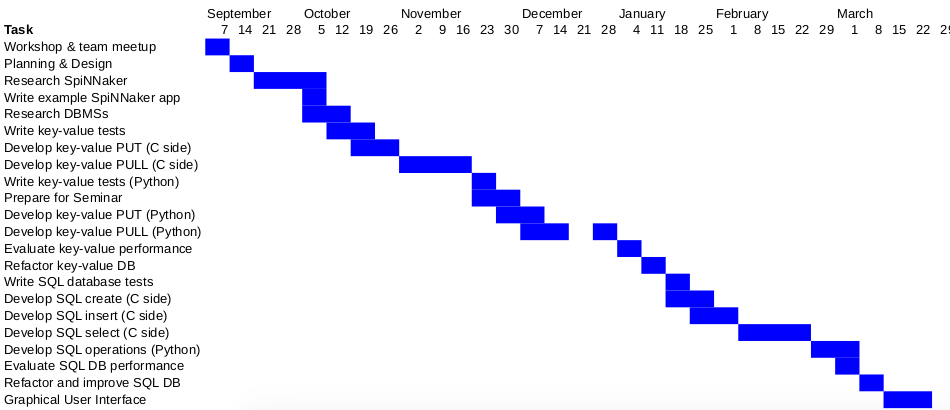
\includegraphics[width=1.3\linewidth, natwidth=950, natheight=410]{images/plan.png}
  \captionof{figure}{Development Plan}
  \label{fig:plan}
\end{figure}

\subsection{Requirements Analysis}
The project plan involved analysing the importance of different requirements based on their relative difficulty and scope within the project aim. Modern database management systems have a broad range of complex requirements. Given the limited resources, I have selected 4 important concepts which must have strict focus on the SpiDB system:

\begin{itemize}
	\item \textbf{Reliability}: user's queries must complete in a reasonable way. This means any internal errors, inconsistencies or communication failures should be handled from within the database system, avoiding unpredicted failures to the user. This is a difficult task given the unreliability of the SpiNNaker communication fabric, earlier discussed on section \ref{sec:comm_fabric}.
	\item \textbf{Durability}: user's queries with the aim of modifying the database state should persist, being internally stored until removal. The SpiNNaker hardware does not contain permanent storage components, reducing this contraint to "insert operations must persist until shutdown". It would be possible to externally connect the board to a mass-storage device, but it is outside of the scope of this project.
	\item \textbf{Isolation}: executing transactions concurrently must have the same effect as doing so sequentially. Concurrency control is an important part of this parallel database system, as it aims to handle thousands of concurrent queries distributed among thousands of processing cores. An approach to ensure isolation in the system is further discussed in section \ref{sec:out-of-order}.
	\item \textbf{Scalability}: the system must be able to handle a large number of parallel queries and have enhanced performance when given more hardware resources, in this case processor count.	This is arguably the most important of all requirements, as the SpiNNaker team is currently focusing on building a large scale machine composed of 1,000,000 processing cores. If this application scales well, it will quickly be able to show the strengths and weaknesses of the machine.
\end{itemize}

These main requirements do not cover two of the four ACID (Atomicity, Consistency, Durability, Isolation) properties of a database: atomicity and consistency. Atomicity, althogh very important on a large commercial application, is extremely hard to achieve in a descentralized system, with the use of complex multi-core rollbacks, and falls out of the scope of this experimental project. Consistency is significant when ensuring data written to the database is valid according to constraints, triggers and cascades, which are originally non-existent in a reduced instruction data store and do not contribute to the project research.

Lastly another outstanding requirement not included in the plan was a strong security protocol. Data encryption and authorization have many advantages, but present themselves as unecessary complexity for a small, private, experimental project.

\subsection{Technologies}
Part of the project plan involves research on the SpiNNaker hardware and API, extensively used on my project. Given the steep learning curve of a low level distributed system, on the 7\textsuperscript{th} of September 2015, I attended the \textit{5\textsuperscript{th} SpiNNaker Workshop}, where tens of researchers from around the globe gathered for a one week course on the SpiNNaker Project in Manchester. I was officially introduced to the team, whom I would learn from and work with for the rest of the year.

The SpiNNaker API is split two: the Python toolchain, running on the \textit{host} machine (user's computer), and C code, compiled to run on the board. The full API can be found at \textit{https://github.com/SpiNNakerManchester}. A strong knowledge of ARM assembly was also needed, given the low level architecture.

These technologies were used to develop the following deliverables:
\begin{itemize}
	\item \textbf{Python}: (2000 lines of code) uploading binaries to the board, status checking, query parsing, Graphical User Interface, data analytics and socket communication.
	\item \textbf{C}: (2500 lines of code) event driven communication between processors, low level memory management, distributed query processing.
\end{itemize}

\section{Design}
Internally, I designed SpiDB to have a hierarchical tree structure architecture, composed of \textit{root}, \textit{branch} and \textit{leaf} nodes/cores. This structure allows a divide-and-conquer approach to the database query plan. When queries are issued by the \textit{host} machine, they are received at the \textit{root} core.

Each chip contains a single \textit{root} node, which handles incomming packets from \textit{host} by redirecting them to \textit{branch} and \textit{leaf} nodes, in an intelligent way, for parallel processing. The middle layer is composed of 4 \textit{branch} cores in charge of aggregating data returned by \textit{leaf} nodes, serving also as "capacitors", slowing down excessive queries which may overload a destination core. Finally the chip is composed of 12 \textit{leaf} nodes, with the aim of actually storing and retrieving database entries (key-value pairs or table rows) on shared memory. These roles can be visualised on figures \ref{fig:tree} and \ref{fig:tree-chip}. The 2 remaining cores are used for internal use of the system (\textit{sark} and \textit{reinjector}), omitted from these figures.

\begin{figure}
\centering
\begin{minipage}{1\textwidth}
  \centering
  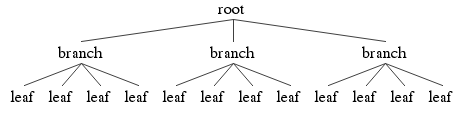
\includegraphics[width=0.9\linewidth, natwidth=618, natheight=120]{images/tree.png}
  \captionof{figure}{SpiDB tree structure}
  \label{fig:tree}
\end{minipage}
\begin{minipage}{1\textwidth}
  \centering
  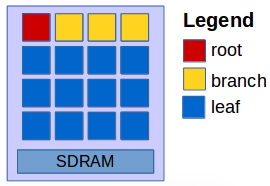
\includegraphics[width=0.5\linewidth, natwidth=270, natheight=186]{images/tree-chip.png}
  \captionof{figure}{Role assignments per chip}
  \label{fig:tree-chip}
\end{minipage}
\end{figure}

There are two important advantages, in favour of scalability, which lead me to make this design choice. Firstly, SpiNNaker communication is unreliable, meaning that a lot of traffic and a central point of failure cause large packet drop rate. This hierarchical structure strongly reduces the problem, and it assures cores will never receive packets from more than 4 other cores, distributing queries in an efficient way and protecting cores from excessive incomming packets. Secondly this approach is inheritably beneficial for merges and aggregation (eg. sql keywords COUNT, MAX, MIN, AVG, SUM, etc.), as these can be done on different layers over iterations. 

A disadvantage of this design is that less cores perform the actual storage and retrival of data. Out of 16 application cores, 4 are used only for distribution of the query plan (\textit{root} and \textit{branches}). This consequently impacts performance, as each \textit{leaf} node will be assigned more memory to read and will be kept busier with query processing.

\section{Implementation}
\label{sec:implementation}

\subsection{Key-value Store}
The first half of the project involved developing a distributed key-value store, in which users can insert and retrieve data entries in a dictionary form. This means the user must be able to set keys mapping to values, both of type \textit{int} or \textit{string}, and retrieve such values when given the same keys. This section describes in detail the internal processing of the insert (\textit{put}) and retrieve (\textit{pull}) queries. 

\subsubsection{PUT}
The \textit{put} operation is the main way of inserting data onto the SpiDB distributed database. 
Upon completion, such operation will store the specified key, mapping to its value, on the memory of an arbitrary chip in the Spinnaker board (as chosen by the \textit{root} core). This operation expects an acknowledgement from the core which stored the entry.

Example usage:
\begin{lstlisting}
put "hello" "world"
put 123 "foo"
put "life" 42
put 1 2
\end{lstlisting}
 
Internally the following steps occur:
\begin{enumerate}
\item User issues query of format \textit{put "key" "value"} on host machine.
\item Query and metadata are converted into a byte array with the following format, transferred via UDP over Ethernet to the board (figure \ref{fig:host-root}).
\lstinputlisting[language=C]{code/putQuery.c}
In this case \textit{SpiDBCommands} is set to the constant representing the put operation, \textit{id} identifies every query uniquely, \textit{info} contains bit encoding of the size and type of both key and value, \textit{k\textunderscore v} contains key and value appended.
\item Packet arrival triggers interrupt on \textit{root} core, via the SDP protocol, and is decoded.
\item \textit{root} selects a \textit{leaf} core to store the data entries in one of the following ways, specified by the user:
\begin{itemize}
	\item \textbf{Naive}: as packets arrive, they are assigned to a different \textit{leaf} node in a Round-Robin manner.
	\item \textbf{Hashing}: the given key is used to produce a 32-bit hash value, which is decoded to assign the query to a specific \textit{leaf} node.
\end{itemize}
\item \textit{root} communicates to chosen \textit{leaf} node with \textit{put} contents via SDP (figure \ref{fig:root-leaf}).
\item \textit{leaf} node triggers an interrupt and stores key-value entry into its dedicated region of SDRAM.
\item \textit{leaf} sends an acknowledgement message over UDP back to host (figure \ref{fig:leaf-host}).
\item User receives timing information and query result.
\end{enumerate}

Complexity: linear to the size of the input key-value, constant to database size.

\begin{figure}
\centering
\begin{minipage}{.32\textwidth}
  \centering
  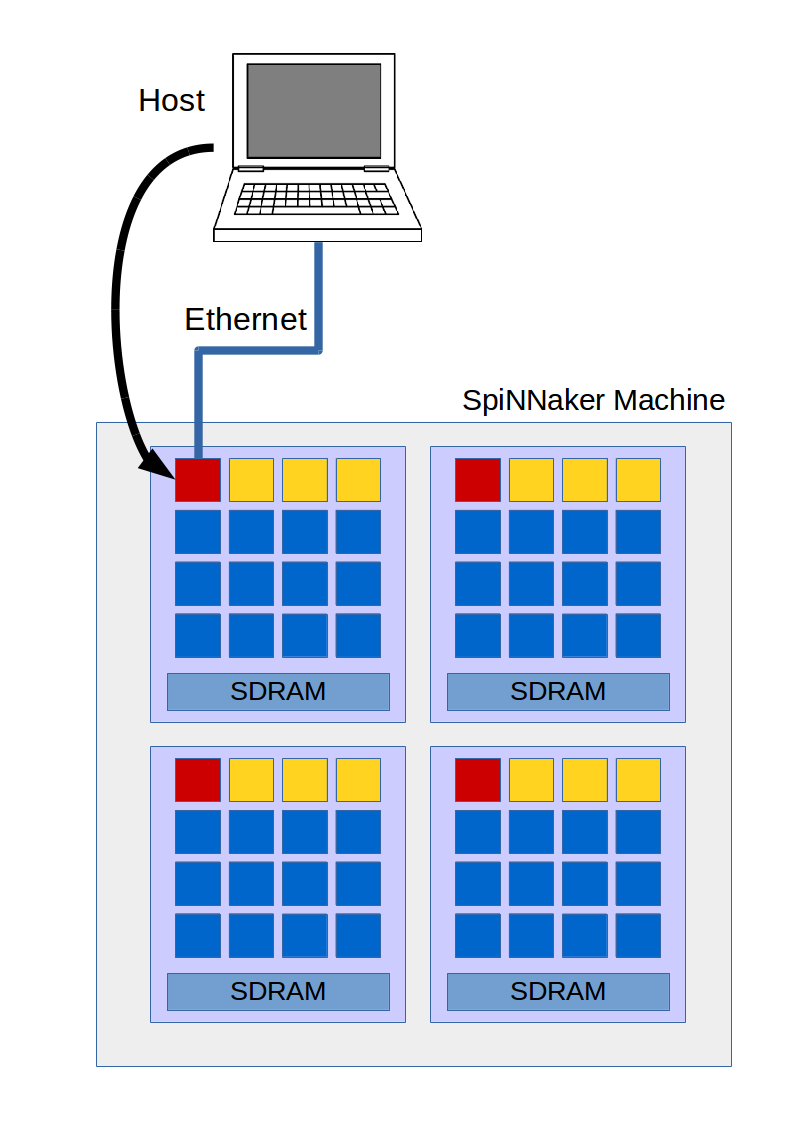
\includegraphics[width=1\linewidth, natwidth=794, natheight=1123]{images/put1.png}
  \captionof{figure}{Host to root packet}
  \label{fig:host-root}
\end{minipage}%
\begin{minipage}{.32\textwidth}
  \centering
  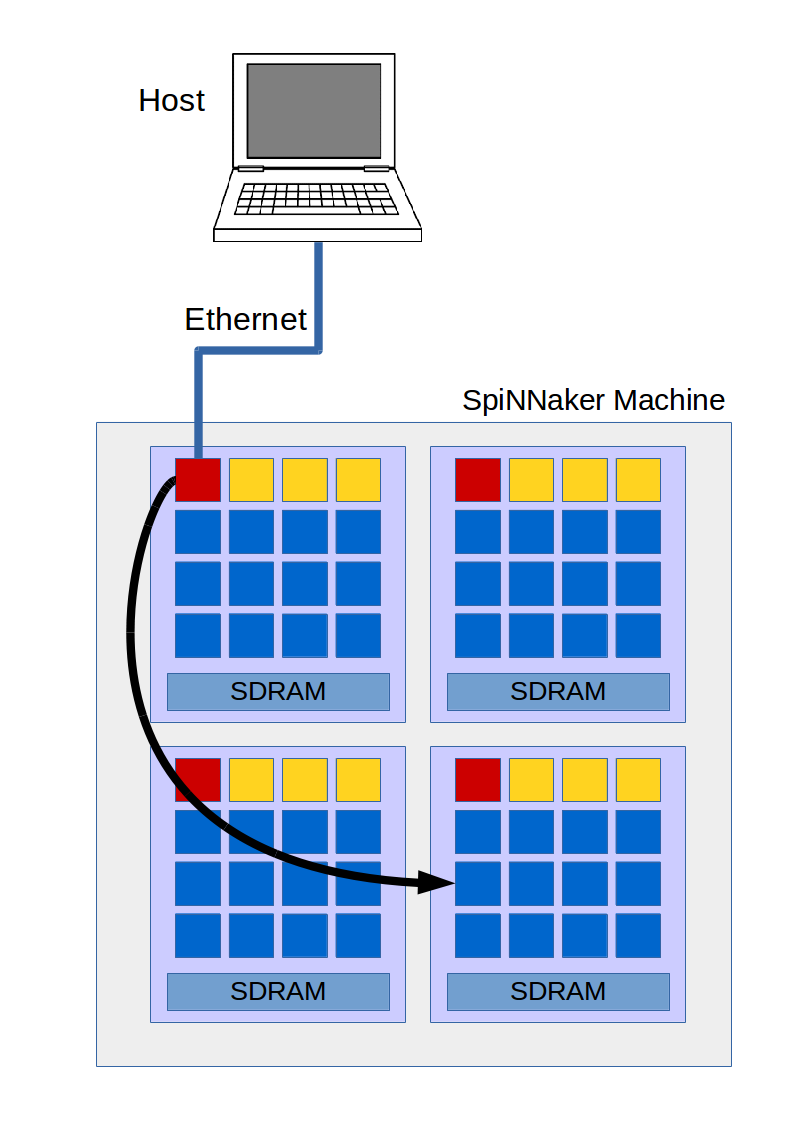
\includegraphics[width=1\linewidth, natwidth=794, natheight=1123]{images/put2.png}
  \captionof{figure}{Root to leaf packet}
  \label{fig:root-leaf}
\end{minipage}
\begin{minipage}{.32\textwidth}
  \centering
  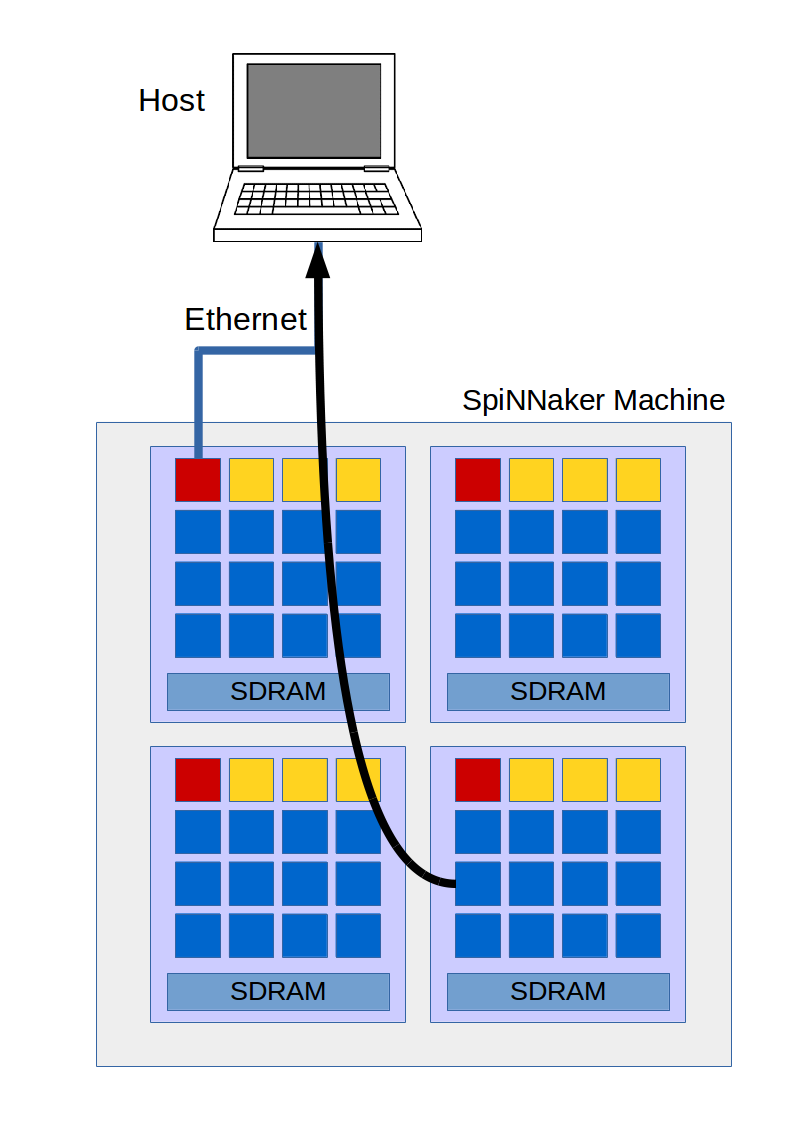
\includegraphics[width=1\linewidth, natwidth=794, natheight=1123]{images/put3.png}
  \captionof{figure}{Leaf to host packet}
  \label{fig:leaf-host}
\end{minipage}
\end{figure}


\subsubsection{PULL}
The \textit{pull} operation is the main way of retrieving data from the SpiDB distributed database. 
Upon completion, such operation will return the value mapped by a given key, from an arbitrary chip in the SpiNNaker board, or not respond if such key was not found. This operation expects a response only if the key is present on the database, thus it is an undecidable problem. The reason for this is further explained in section \ref{sec:unreliable_comm}.

Example usage:
\begin{lstlisting}
pull "hello"
pull 123
\end{lstlisting}

Internally the following steps occur:
\begin{enumerate}
\item User issues query of format \textit{pull "key"} on host machine.
\item Query and metadata are converted into a byte array with the following format, transferred via UDP over Ethernet to the board %(figure \ref{fig:host-root}).
\lstinputlisting[language=C]{code/pullQuery.c}
Where \textit{SpiDBCommands} represents the pull operation constant, \textit{id} is the query, \textit{info} contains bit encoding of the size and type of the given key, \textit{k} contains the key itself encoded as a byte-array.
\item Packet triggers interrupt on \textit{root} core, via SDP, and is decoded.
\item \textit{root} selects one of the following search strategies, based on database type:
\begin{itemize}
	\item \textbf{Naive}: there is no knowledge of which, if any, chip contains the given key. Therefore \textit{root} issues a multicast packet to all \textit{leaf} nodes on the board, requesting them to linearly scan their regions of shared memory, searching for the entry.
	\item \textbf{Hashing}: the key is used to produce a 32-bit hash value, which, if existent on the database, must be present at the memory of a specific core, pointed by the decoding of such hash value. Therefore \textit{root} node sends a single SDP packet to chosen \textit{leaf}, requesting it to search for the given key.
\end{itemize}
\item Each \textit{leaf} node that received a search request triggers an interrupt and searches for key-value mapping in SDRAM memory. If key is found, value is returned over UDP back to host.
\item User receives timing information and query result.
\end{enumerate}

Complexity: linear to the size of the input, linear to database size.

Algorithms \ref{alg:root} and \ref{alg:leaf} show a high level simplification of code running in the \textit{root} and \textit{leaf} nodes, as described above, through the event driven application, implementing \textit{put} and \textit{pull} operations.

\begin{algorithm}
\caption{Root core}
\label{alg:root}
\begin{algorithmic}[1]
\Procedure{onReceive}{$sdp$}
	\If{$sdp.command$ \textbf{is} $PUT$}
		\If{$DB\_TYPE$ \textbf{is} $NAIVE$}
			\State forward $PUT$ query to next core (Round-robin)
		\ElsIf{$DB\_TYPE$ \textbf{is} $HASH$}
			\State $h \gets hash(sdp.key)$
			\State $chipx \gets h[0:7]$
			\State $chipy \gets h[8:15]$
			\State $core \gets h[16:24]$
			\State forward sdp $PUT$ query to (chipx, chipy, core)
		\EndIf
	\EndIf

	\If{$sdp.command$ \textbf{is} $PULL$}
		\If{$DB\_TYPE$ \textbf{is} $NAIVE$}
			\State issue multicast $PULL$ to all cores in the system
		\ElsIf{$DB\_TYPE$ \textbf{is} $HASH$}
			\State $h \gets hash(sdp.key)$
			\State $chipx \gets h[0:7]$
			\State $chipy \gets h[8:15]$
			\State $core \gets h[16:24]$
			\State forward sdp $PULL$ query to (chipx, chipy, core)
		\EndIf
	\EndIf
\EndProcedure
\end{algorithmic}
\end{algorithm}

\begin{algorithm}
\caption{Leaf core}
\label{alg:leaf}
\begin{algorithmic}[1]
\Procedure{onReceive}{$sdp$}
	\If{$sdp.command$ \textbf{is} $PUT$}
		\State store $sdp.key$ and $sdp.value$ in SDRAM
	\EndIf

	\If{$sdp.command$ \textbf{is} $PULL$}	
		\State $entry \gets SDRAM[0]$
		\State $i \gets 0$		
		
		\While{$entry$ \textbf{is not null}}
			\If{$entry.key$ \textbf{is} $sdp.key$}
				\State send response to host with $sdp.value$
				\State \textbf{return}
			\EndIf
			\State $entry \gets SDRAM[i]$
			\State $i \gets i+1$
      	\EndWhile
	\EndIf
\EndProcedure
\end{algorithmic}
\end{algorithm}

\subsection{Relational Database}
The second half of the project involves developing an SQL-based distributed database on top of the key-value store layer. Entries are stored in a structured way, bounded by the definition of tables. In this RDMS users can create tables with different fields, insert values and retrieve them with given conditions. This section describes in detail the internal processing of the \textit{create}, \textit{insert} and \textit{select} queries. 

\subsubsection{CREATE}
In SpiDB, the \textit{create} operation is used to generate a table definition in the SpiNNaker hardware. Data can only be inserted into the database if a corresponding table exists. This query has as parameters the table name, field names and their types (\textit{int} or \textit{string}). Multiple distinct tables can be issued symultaneously, although they are handled by a single core. 
This operation expects an acknowledgement from the \textit{root} core, which sets the failure flag if the table definition already exists.

Example usage:
\begin{lstlisting}
CREATE TABLE Dogs(name varchar(10), owner varchar(35), age integer);
CREATE TABLE People(name varchar(35), lastname varchar(20));
\end{lstlisting}

Internally the following steps occur:
\begin{enumerate}
\item User issues query of format \textit{CREATE TABLE name(column1 type(size), ...)} on host machine.
\item Query and metadata are converted into a byte array and sent to the board (format can be found on appendix section \ref{sec:appendix-queries}).
\item \textit{root} core receives and decodes SDP packet.
\item If table does not exist on the database yet, \textit{root} core stores table definition and metadata in its region of shared SDRAM, accessible by other cores for insert/retrieve operations. 
\item \textit{root} core sends acknowledgement back and information is displayed to the user.
\end{enumerate}

Complexity: linear to the size of the input, constant to database size.
   
\subsubsection{INSERT}
New values can be added to the database management system through the \textit{INSERT} query. A single entry is an \textit{int} or \textit{string} value assigned to a column on a given table at a new row. Multiple entries can be safely inserted concurrently, as they are distributed across different cores. This operation expects an acknowledgement from the \textit{leaf} node in charge of storing the value and metadata, with the failure flag set if memory is full.

Example usage:
\begin{lstlisting}
INSERT INTO Dogs(name,owner,age) VALUES ("Toddy","Arthur",8);
INSERT INTO Dogs(name,owner,age) VALUES ("Guto","Arthur",10);
INSERT INTO People(name,lastname) VALUES ("Arthur","Ceccotti");
INSERT INTO People(name,lastname) VALUES ("Canny","Dattlin");
\end{lstlisting}

Internally the following steps occur:
\begin{enumerate}
\item User issues query of format \textit{INSERT INTO table(column1, ...) VALUES (value1, ...)} on host machine.
\item Query is broken down into column-value pairs, containing also value type, size and specified table (eg. ["name":("Arthur", type: string, size: 6)]). This step is necessary because SDP packets have a limit size of 256-bytes, thus not being able to carry one single large packet containing all the assignments for a table row. Streaming smaller packets also decreases the need for a large storage buffer at the destination.\cite{sdp}
\item Column-value pairs (entries) are converted into a byte array, sent to the board, being received and decoded by the \textit{root} node.
\item The column-value pair query is forwarded to a \textit{leaf} node in a Round-Robin way.
\item \textit{leaf} node receives query, checks if specified table exists in shared memory SDRAM and reads its definition.
\item \textit{leaf} node stores column-value pair into a new row in reserved region for given table. The SpiDB RDMS is row-based, thus entire rows are stored consecutively in a structured way at all cores.
\item \textit{leaf} node acknowledges query, returned to the user.
\end{enumerate}

Complexity: linear to the size of the input, constant to database size.

\subsubsection{SELECT}   
In the SpiDB system, multiple entries from a table can be retrieved using the \textit{SELECT} query, following the standard SQL syntax. Selection criteria can be specified by the user and matching results are streamed until a timeout is reached. If no value in the table matches such criteria, there will be no response from the board, which is a consequence of not making use of internal acknowledgements, as discussed in section \ref{sec:unreliable_comm}. This is a similar behaviour to \textit{pull} requests. 

The select query has the capability of producing a very large amount of traffic in the system, as it is the only query with a variable number of packets returned. All other queries have at most one acknowledgement per incomming packet. 

Example usage:
\begin{lstlisting}
SELECT name FROM Dogs WHERE owner = "Arthur";
SELECT name, owner FROM Dogs;
SELECT * FROM People WHERE age > 5 and age < 20;
SELECT lastname FROM People WHERE name = lastname;
\end{lstlisting}
   
Internally the following steps occur:
\begin{enumerate}
\item User issues query of format \textit{SELECT *\textbar fiel1, ... FROM table WHERE condition}, which is converted and sent as a single packet to the SpiNNaker board.
\item Upon receival, \textit{root} node issues a multicast packet to every \textit{leaf} node on the board, requesting search for all rows which match the WHERE criteria.
\item Every \textit{leaf} node linearly checks appropriate condition and forwards matching column-value pairs on packets to their appropriately assigned \textit{branch} nodes.
\item \textit{branch} nodes aggregate fields if requested, controls speed of execution and sends packet to host with such entry definition.
\item User receives an arbitrary amount of entries, displayed as a table of results.
\end{enumerate}

Complexity: linear to the size of the input, linear to database size.
 
\subsection{User Interface} 
Although a graphical user interface was not an essential part of the project plan, a simple one was created for the purposes of demonstration, data plotting and ease of visualization. By making use of the SpiDB API, the UI includes features to import \textit{sql} files, ping the board, issue concurrent queries, visualize previous queries, display result statistics and graphs. An example instance can be seen in figure \ref{fig:gui}.

\begin{figure}
\center
  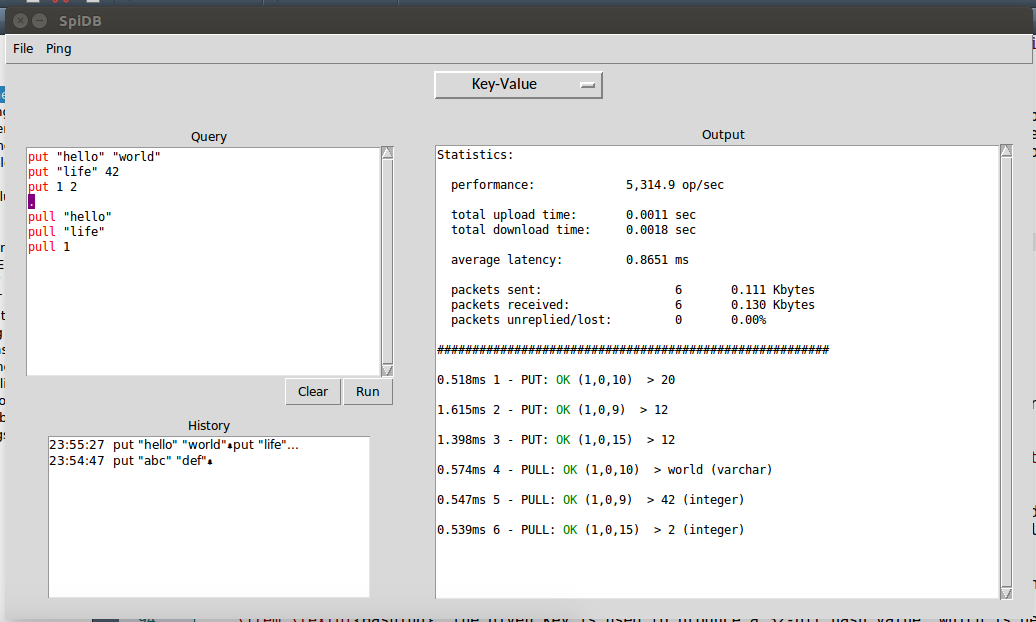
\includegraphics[width=1\linewidth, natwidth=1036, natheight=622]{images/GUI.png}
  \captionof{figure}{Graphical User Interface}
  \label{fig:gui}
\end{figure}

\section{Testing and Debugging}
I started the project with a Test-Driven Development approach, writing Python tests with the \textit{unittest} module and C assertions with part of the SpiNNaker API module \textit{debug.h} and my own code. This allowed high reliability from the start. Running tests can be seen in figure \ref{fig:testing}. Testing and development was done from the bottom up, starting from internal memory management, core communication and finally the user interface and host communication.
Testing involved initially a number of insert queries with different types and sizes. Given the SpiNNaker architecture is word aligned, it was important to test boundaries along data sizes along multiples of 4 bytes. Examples of tests run can be seen on table \ref{table:tests}.
Both the key-value store and the SQL-RDMS were also tested for their performance and scalability, running over 100,000 symultaneous incomming queries with real data pulled from a modern English vocabulary. The results from these experiments can be read on chapter \ref{cha:eval}.

\begin{table}
\begin{tabular}{ l | l | l | l | l }
\textbf{Operation} & \textbf{arg1} & \textbf{arg2} & \textbf{expected result} & \textbf{reason} \\
PUT & "hello" & "world" & success & \\
PUT & "foo" & "bar" & success & \\
PUT & "A" & "B" & success & \\
PUT & 42 & "life" & success & \\
PUT & "abc" & 123 &  success & \\
PUT & 1 & 2 & success & \\
PUT & 1.5 & 2.5 & failure & no floating point support\\
PUT & "hello" & "earth" & failure & key already exists \\
PUT & (very long string) & "value" & failure & 256-byte limit for now \\
PUT & (very long int) & "value" & failure & 256-byte limit for now \\
PUT & (empty) & "string" & failure & both key and value must be set \\
PUT & "\begin{CJK*}{UTF8}{bsmi}你\end{CJK*}" & "\begin{CJK*}{UTF8}{bsmi}好\end{CJK*}" & failure & ASCII support only \\
PULL & "hello" & & "world" & \\
PULL & 42 & & "life" & \\
PULL & "abc" & & 123 & \\
PULL & "HELLO" & & failure & case sensitive \\
PULL & (very long string) & & failure & 256-byte limit for now \\
PULL & "a new key" & & failure & key does not exist \\
\end{tabular}
\caption{Examples of Key-value store test cases}
\label{table:tests}
\end{table}

Realtime debugging on the SpiNNaker board is relatively hard, but luckly the API provides ways to log messages in each core's private data memory, which can be read by an external process upon execution of the program. Debugging was performed with a tool named \textit{ybug} (\textit{https://github.com/SpiNNakerManchester/ybug}), also developed by the team, which allows core status checking, uploading binaries, reading logs and memory content, among other functionality.\cite{ybug} On the \textit{host} Python code, debugging was done using the Pycharm IDE runtime tools.

\begin{figure}
  \centering
  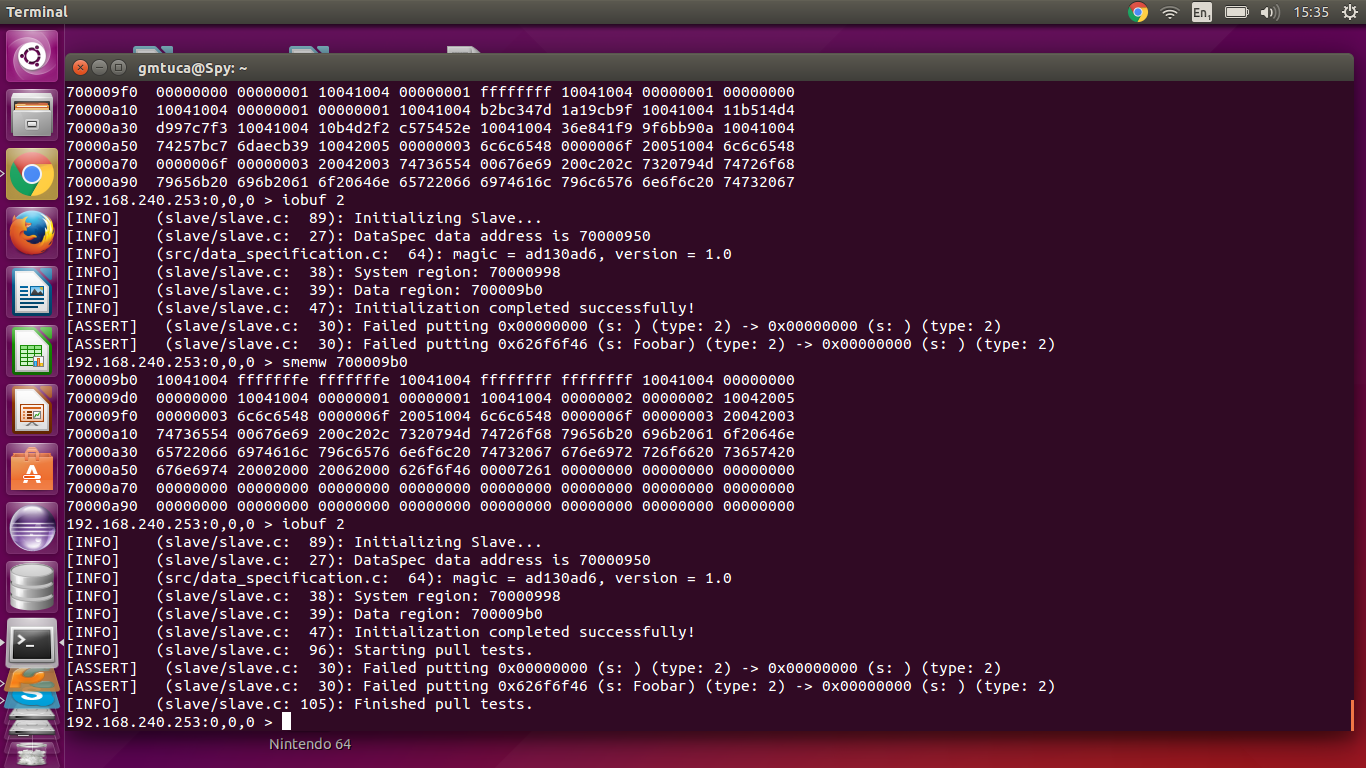
\includegraphics[width=1.15\linewidth, natwidth=1366, natheight=768]{images/debugging.png}
  \captionof{figure}{Debugging}
  \label{fig:debugging}
  \centering
  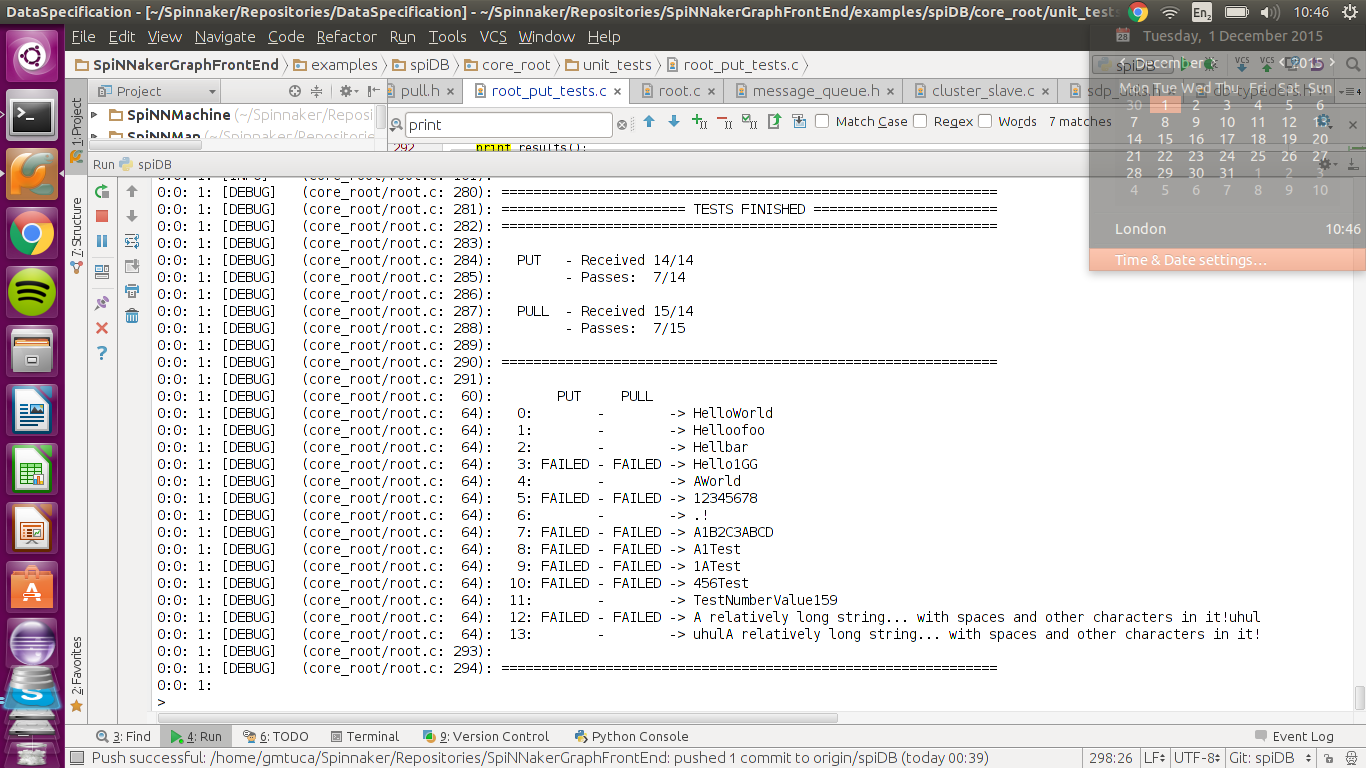
\includegraphics[width=1.15\linewidth, natwidth=1366, natheight=768]{images/testing.png}
  \captionof{figure}{Testing}
  \label{fig:testing}
\end{figure}

\section{Challenges}
This section outlines a list of different challenges and problems I had to face during the development of the application and how they influenced decision making.


\subsection{Out-of-order execution}
\label{sec:out-of-order}
A multi-threaded system must account for the fact that queries may not be executed in the order they are issued, which can be a concern depending on the application. As SpiNNaker is a distributed architecture, it cause problems and inconsistencies.
For example, using SpiDB, if we try to execute the following code sequence in order:\\
\begin{lstlisting}[caption={Non-blocking execution}, label=list:non-blocking]
put "hello" "world"
pull "hello"
\end{lstlisting}

We are not guaranteed that the \textit{pull} query will retrieve the value "world". As both queries are executed symultaneously on the SpiNNaker board, there is a chance that the \textit{pull} operation will terminate before the \textit{put} does, thus failing to return a value.

As a solution to this dependency constraint, my SpiDB database API includes the syntax symbol "." (dot) which blocks execution until all preceeding operations terminate. This allows the programmer to control execution flow, choosing what is allowed to compute out-of-order (in parallel) and what should be sequentialised at a cost of performance. This is a similar concept to the Verilog blocking and non-blocking assignments.

\begin{lstlisting}[caption={Blocking execution}, label=list:blocking1]
put "hello" "world"
.
pull "hello"
\end{lstlisting}

The above code will assure sequential code, meaning the \textit{pull} operation will always return "world". It is usually a good idea to block execution when given a dependency constraint. This can also be done with larger code fragments.

\begin{lstlisting}[caption={Blocking execution}, label=list:blocking2]
put "hello" "world"
put "life" 42
put 123 456
.
pull "hello"
pull "life"
pull 123
\end{lstlisting}

It is worth noting that although non-block operations can cause out-of-order execution, it does not occur very frequently. This is because, when transmitting data to the board, queries are serialised over ethernet in order of appearence and in addition there is a small forced transmission delay between these packets. This will be further discussed on chapter \ref{cha:eval}.

\subsection{Unreliable communication}
\label{sec:unreliable_comm}

The SpiNNaker communication protocol can be unreliable, as packets are not guaranteed to arrive at destination, as discussed earlier in section \ref{sec:comm_fabric}. This effect is worsen when there is large traffic in the system, so the more packets are being sent, the more packets are lost. While developing the application I had to consider this cost, assuring reduced communication when possible. 

Queries such as \textit{put} issue only one packet at a time, allowing an end-to-end acknowledgement without significant packet drops or performance costs. For this reason the \textit{put} query, alongside the SQL commands \textit{create} and \textit{insert} always expect a response, which contains timing information and a flag whether it was successful or not. The steps of running SpiDB queries can be revised in section \ref{sec:implementation}.

On the other hand the \textit{pull} and \textit{select} commands issue multicast packets (one-to-many). This means for each query, a packet is sent to up to hundreds of codes, which SpiNNaker is particularly optimized for, but the opposite (many-to-one) is more difficult. Multiple cores sending \textit{SDP} packets to a single core results on a very large packet drop. Only a total of 4 of these packets arrive successfully, as it is the limit of \textit{SDP} channels per core. In the worst case, too many packets have also the capability of crashing the destination core.
This means when a packet has multiple destinations, acknowledgements would worsen the situation, as most of these would be dropped and it would highly increase traffic in the system, which itself is a reason for packet loss.

This analysis has lead me to make the design decision of not using internal acknowledgements for every packet sent. In \textit{pull} queries, \textit{leaf} nodes only respond when they have found the specified key, which means there will be at most one acknowledegement. If the key is not found on the database, not a single \textit{leaf} core will respond, which can only be known externally with the use of a timeout.

The advantage of this approach is that it increases speed of execution for successful queries and avoids excessive traffic in the system, increasing reliability. This comes at the cost of slow execution of instances of \textit{pull} requests where the key does not exist on the database. Using this approach performance is poor when requested entries do not exist. Assuming most of the time users will try to retrieve entries previously inserted on the database, I evaluate this decision to be wise.

\subsection{API Bugs}
I have been one of the few users of a large amount of the SpiNNaker API, currently under contruction. This means some of it has not been fully tested, resulting in strange behaviour at times, making debugging of my own application difficult. Besides aiming to gather benchmarks for SpiNNaker, my project itself has been very useful when exposing unexpected errors or inconsistencies in the team's codebase.

Facing these issues was certainly a challenge, as they belonged to domains I had little knowledge of. I was a good opportunity for me to learn and improve code quality of a large, collaborated project, by testing its usability and evaluating its outputs. This means my project involved not only developing the database application, but also collaborating to improve SpiNNaker itself.

The main API bugs I exposed and helped resolve were:

\begin{itemize}
\item \textbf{Duplicate packets}: when multiple distinct SDP packets were sent from different sources to the same destination, strangely the receiving core would read the same packet duplicated a number of times. This behaviour was highly unexpected to the team, so upon extensive testing, I was able to point the issue to a running processor named \textit{reinjector}, in charge of re-issuing lost packets, and resolve the problem. 
\item \textbf{Data Specification Error}: when uploading binaries to the board, sometimes cores would crash with an internal error state (SWERR), upon evaluating and providing the team with detailed feedback on the issue, I found this to be caused by the SpiNNaker Data Specification framework, which handles allocation of data in shared RAM.

% \item algorithms
\end{itemize}




